% Introduction

\chapter{Introduction}

Specialized hardware for running deep learning algorithms seems to be a natural step in the evolution of
Artificial Intelligence.  Google, for example, developed its own \gls{asic} named \gls{tpu}
to accelerate tensor computations. The formidable cost of such endeavors limits \gls{asic} development to
the big players in the industry. For tech startups and hobbyists, the \gls{fpga} comes to rescue by filling
the gap between high-cost customized ICs and the need to make specialized hardware for certain
applications. The programmable logic blocks contained in the \gls{fpga} can be reconfigured, making it
ideal for situations where "`in the field"' functionality update is required. It is also a valuable tool
for fast prototyping and verification of \gls{asic} design with low cost.

Given a phenomenon, a discriminative model takes data that can be observed from the phenomenon and outputs
data that can only be inferred. For instance, let the phenomenon be a group of people speaking different
languages, a discriminative model can take the speech data and infer the language being spoken. In other
word, the model classifies the speeches into different language types or labels. This can be done, e.g.,
by analyzing the linguistic models of each speech and observe the differences. By contrast, a generative
model outputs both data that can be directly observed as well as data that can only be inferred. Therefore,
in the previous example, a generative model would have to learn each language and be able to generate
speeches of them. Probabilistically speaking, a discriminative model learns the conditional probability
distribution $P(Y \mid X)$ (the probability of language $Y$ given speech $X$), while a generative model
learns the joint probability distribution $P(X,Y) = P(X \mid Y)P(Y)$, which explicitly models the speech
generation process of each language class.

Generative models are interesting since they are capable of creating new data that resembles the real world
data. These models enable the machine to paint new paintings, compose new music, or write new poetries.
Many types of generative models exist, including deep belief networks, variational autoencoder,
Boltzmann machine, \gls{gan}s, etc. A \gls{gan} model consists of two different neural networks trained to
compete against each other in order to learn about the probability distribution of a particular dataset.
The training process pits the two players in a minimax game so that the performance of both networks improves
over time. Introduced in 2014 by Ian Goodfellow \textit{et al}. \cite{goodfellow:gan}, it soon gained
popularity in the machine learning community, kindled a wave of research on improving the training properties
and quality of generation.

The marriage of \gls{fpga} and \gls{gan} seems to be an interesting topic in its own right. This project
explores such possibilities by implementing a pre-trained generator model of \gls{dcgan} proposed by
Alec Radford \textit{et al}. \cite{radford:conv_gan} on \gls{fpga} to generate realistic pictures.
Figure \ref{fig:bedroom} shows a group of generated images of bedrooms.

\begin{figure}[h]
  \centering
  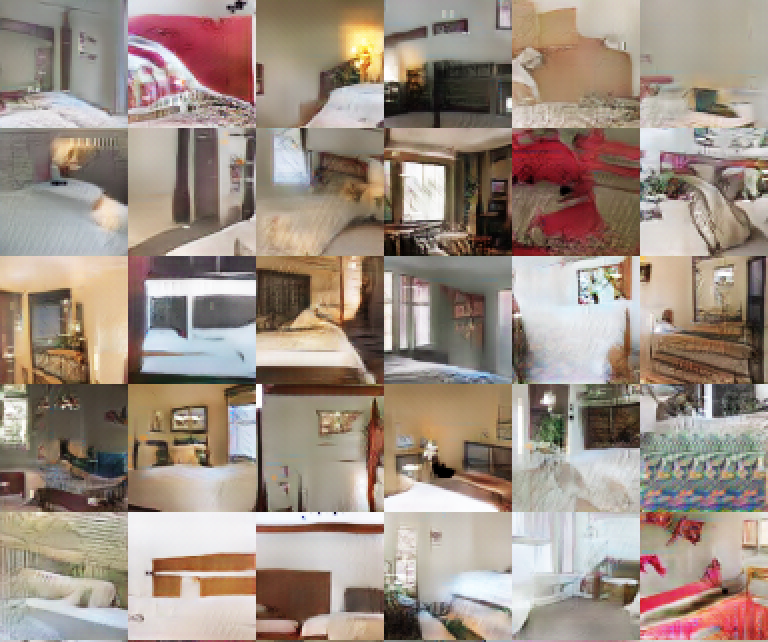
\includegraphics[scale=0.5]{bedroom}
  \caption{Images of bedrooms generated by DCGAN \cite{radford:conv_gan}}
  \label{fig:bedroom}
\end{figure}

Nowadays \gls{hls} is a quite popular option for implementing algorithms on \gls{fpga}. \gls{hls} takes a
behavioral description written in a high-level programming language such as C and translates the description
into \gls{rtl} \gls{hdl} such as Verilog or VHDL. This approach is particularly favored by software
engineers who wish to quickly convert a software program into hardware implementation. In this project,
however, low-level HDL was chosen to implement the generator model to gain finer control of the implementation
details. A naïve Verilog version was implemented first, then several optimization possibilities were
experimented. This paper serves as a rather detailed documentation of the design and implementation process.
The source code of this project is published on GitHub \cite{github:dcgan_fpga} under Apache License 2.0.

The generator is a deep \gls{cnn}. In such networks a large part of the computation is done with an
operation called the \gls{gemm}. Therefore, an efficient implementation of \gls{gemm} is crucial to the
acceleration. However, CNNs are normally implemented with floating-point numbers, which are usually less
efficient to handle in hardware than fixed-point numbers. If only we could carry out the computation in
fixed-point numbers and then convert the result back to floating-point numbers! Such techniques do exist
and they are referred to as quantization, which is the key to realize high performance in hardware. Chapter 5
provides a detailed discussion of the quantization scheme used in this project.

\clearpage %force the next chapter to start on a new page. Keep that as the last line of your chapter!
